\documentclass[aspectratio=169, 9pt]{beamer}

% ==============================================================================
% THEME & NAVIGATION CONFIGURATION
% ==============================================================================
\usetheme[sectionpage=none]{metropolis}
\useoutertheme[subsection=false]{miniframes}
\nonstopmode

% ==============================================================================
% REQUIRED PACKAGES
% ==============================================================================
\usepackage{bookmark}
\usepackage{tikz}
\usetikzlibrary{shapes.geometric, arrows.meta, positioning, calc, shadows.blur, fadings}

\usepackage[utf8]{inputenc}
\usepackage[T1]{fontenc}
\usepackage{lmodern}
\usepackage{graphicx}
\graphicspath{{../assets/}{assets/}{templates/assets/}{../../templates/assets/}{./}}

\usepackage[backend=biber, style=numeric, sorting=none, maxnames=2, natbib=true, doi=false, url=false, isbn=false]{biblatex}
\addbibresource{references.bib}

\usepackage[most]{tcolorbox}
\usepackage{booktabs}
\usepackage{array}
\usepackage{colortbl}
\usepackage{listings}
\usepackage{amsmath, amssymb, amsfonts}

% ==============================================================================
% COLOR PALETTE (Editorial Crimson, Slate & Forest Green)
% ==============================================================================
\definecolor{background}{RGB}{255, 255, 255}
\definecolor{foreground}{RGB}{30, 30, 40}
\definecolor{accent}{RGB}{220, 40, 40}
\definecolor{structure}{RGB}{50, 50, 60}
\definecolor{journalblue}{RGB}{26, 82, 118}
\definecolor{midorange}{RGB}{243, 156, 18}
\definecolor{donegreen}{RGB}{46, 139, 87}
\definecolor{tableheader}{RGB}{240, 244, 248}

\setbeamercolor{normal text}{fg=foreground, bg=background}
\setbeamercolor{alerted text}{fg=accent}
\setbeamercolor{frametitle}{fg=foreground, bg=background}
\setbeamercolor{title separator}{fg=accent}
\setbeamercolor{section in head/foot}{fg=foreground, bg=structure!6}
\setbeamercolor{mini frame}{fg=accent, bg=structure!25}

\setbeamerfont{frametitle}{size=\large, series=\bfseries}
\setbeamerfont{title}{size=\Large, series=\bfseries}
\setbeamerfont{subtitle}{size=\normalsize}

% Progress Bar Header
\setbeamertemplate{headline}{%
  \begin{beamercolorbox}[wd=\paperwidth]{section in head/foot}
    \vskip3pt\centering
    \insertnavigation{0.7\paperwidth}%
    \vskip3pt%
  \end{beamercolorbox}%
  {\color{accent}\hrule height 2pt}%
}

% Minimalist Page Number Footer
\setbeamertemplate{footline}{%
  \vspace{3pt}%
  \hfill\usebeamercolor[fg]{page number in head/foot}\usebeamerfont{page number in head/foot}\insertframenumber\hspace*{1.2em}\vspace{3pt}%
}

% UI Helpers
\setbeamertemplate{itemize item}{\raisebox{0.18ex}{\textcolor{accent}{\rule{0.38em}{0.38em}}}}
\setbeamertemplate{itemize subitem}{\raisebox{0.15ex}{\textcolor{accent!60}{\rule{0.28em}{0.28em}}}}
\setlength{\labelsep}{0.5em}

\newtcbox{\pill}{on line, enhanced, colframe=accent, boxrule=0pt, arc=2.5pt,
  interior style={top color=accent, bottom color=accent!85},
  coltext=white, left=4pt, right=4pt, top=1.2pt, bottom=1.2pt,
  fontupper=\fontsize{6pt}{7pt}\selectfont\bfseries\sffamily}

\newtcbox{\pillalt}{on line, enhanced, colframe=structure, boxrule=0pt, arc=2.5pt,
  interior style={top color=structure!85, bottom color=structure!70},
  coltext=white, left=4pt, right=4pt, top=1.2pt, bottom=1.2pt,
  fontupper=\fontsize{6pt}{7pt}\selectfont\bfseries\sffamily}

\newtcolorbox{takeaway}[1][]{enhanced, colframe=accent, boxrule=0pt, leftrule=2.5pt,
  interior style={left color=accent!10, right color=accent!2},
  arc=1.5pt, outer arc=1.5pt, left=5pt, right=5pt, top=3pt, bottom=3pt,
  fontupper=\scriptsize, before skip=3pt, after skip=2pt, #1}

\newcommand{\kpicard}[3]{%
  \begin{tcolorbox}[enhanced, colframe=structure!20, colback=structure!3, boxrule=0.5pt, arc=2pt,
    left=3pt, right=3pt, top=2.5pt, bottom=2.5pt, halign=center]
    {\fontsize{6pt}{7pt}\selectfont\bfseries\textcolor{structure}{#1}}\\[1pt]
    {\normalsize\bfseries\textcolor{accent}{#2}}\\[1pt]
    {\tiny\textcolor{structure!70}{#3}}
  \end{tcolorbox}%
}

% ==============================================================================
% PRESENTATION METADATA
% ==============================================================================
\title{Quantitative Biophysics and Ecological Dynamics}
\subtitle{Bio-Energetics, Native TikZ Trophic Pyramids, and Enzymatic Kinetics}
\author{Dr.~Jordan Taylor \and Prof.~Alex Morgan}
\institute{Institute for Quantitative Biology \& Division of Ecology}
\date{\today}

\setbeamertemplate{title page}{
  \vfill
  \centering
  
\includegraphics[height=1.3cm]{university_seal.jpg}\par\vspace{0.4em}
  \usebeamerfont{title}\inserttitle\par
  \vspace{0.2em}
  \usebeamerfont{subtitle}\textcolor{structure}{\insertsubtitle}\par
  \vspace{0.5em}
  {\color{accent}\rule{0.75\textwidth}{1.2pt}}\par
  \vspace{0.5em}
  \usebeamerfont{author}\insertauthor\par
  \vspace{0.2em}
  \usebeamerfont{institute}\textcolor{structure!75}{\insertinstitute}\par
  \vspace{0.2em}
  \usebeamerfont{date}\textcolor{structure!55}{\insertdate}\par
  \vfill
}

% ==============================================================================
% DOCUMENT BEGIN
% ==============================================================================
\begin{document}

% --- Slide 1: Title ---
\begin{frame}[plain]
    \titlepage
\end{frame}

% --- Slide 2: Roadmap ---
\section{Roadmap}
\begin{frame}{Biophysical Curriculum \& Ecological Scope}
    \begin{columns}[c]
        \begin{column}{0.48\textwidth}
            \pillalt{CURRICULUM}\par\vspace{0.3em}
            \begin{itemize}\setlength{\itemsep}{2.5pt}
                \item \textbf{1. Bio-Energetic Laws:} Lindeman efficiency and solar assimilation~\cite{lindeman1942trophic}.
                \item \textbf{2. Trophic Systems:} Energy tier pyramids and thermodynamic loss.
                \item \textbf{3. Food Web Cascades:} Top-down vs bottom-up regulation~\cite{begon2006ecology}.
                \item \textbf{4. Enzymatic Kinetics:} Michaelis-Menten and Hill cooperativity~\cite{keener2009mathematical}.
                \item \textbf{5. Population Dynamics:} Lotka-Volterra predator-prey systems.
            \end{itemize}
        \end{column}
        \begin{column}{0.48\textwidth}
            \begin{takeaway}
                \textbf{\textcolor{accent}{Core Principle:}} Energy transfer across biological hierarchies obeys strict thermodynamic conservation laws.
            \end{takeaway}
            \vspace{0.4em}
            \begin{columns}[c]
                \begin{column}{0.48\textwidth}
                    \kpicard{EFFICIENCY}{$\lambda \approx 10\%$}{Trophic Transfer}
                \end{column}
                \begin{column}{0.48\textwidth}
                    \kpicard{HEAT DISSIPATION}{$90\%$}{Metabolic Loss}
                \end{column}
            \end{columns}
        \end{column}
    \end{columns}
\end{frame}

% --- Slide 3: Trophic Energy Flow & Bio-Energetics ---
\section{Bio-Energetics}
\begin{frame}{Ecological Energy Flow: Lindeman's 10\% Law}
    \begin{columns}[t]
        \begin{column}{0.48\textwidth}
            \pillalt{THERMODYNAMICS}\par\vspace{0.2em}
            \scriptsize
            \textbf{1. Lindeman Trophic Efficiency Rule:}
            \begin{equation*}
                E_{n+1} = \lambda \cdot E_n, \quad \text{where } \lambda \approx 0.10
            \end{equation*}
            \vspace{0.1em}
            \textbf{2. Bio-Energetic Budget Equation:}
            \begin{equation*}
                \frac{dB}{dt} = \text{Assimilation} - \text{Respiration} - \text{Excretion}
            \end{equation*}
            \begin{itemize}\setlength{\itemsep}{1.5pt}
                \item \textbf{Gross Primary Productivity (GPP):} Total solar energy captured.
                \item \textbf{Net Primary Productivity (NPP):} $\mathrm{NPP} = \mathrm{GPP} - R_{\mathrm{autotroph}}$.
            \end{itemize}
        \end{column}
        \begin{column}{0.48\textwidth}
            \pill{TROPHIC CASCADE}\par\vspace{0.2em}
            \scriptsize
            \textbf{Tier Biomass Quantities:}
            \begin{itemize}\setlength{\itemsep}{2pt}
                \item \textbf{Apex Predators (Tier 4):} $10\,\mathrm{J}$ (Hyper-carnivores).
                \item \textbf{Secondary Consumers (Tier 3):} $100\,\mathrm{J}$ (Carnivores).
                \item \textbf{Primary Consumers (Tier 2):} $1{,}000\,\mathrm{J}$ (Herbivores).
                \item \textbf{Primary Producers (Tier 1):} $10{,}000\,\mathrm{J}$ (Plants).
            \end{itemize}
            \vspace{0.2em}
            \begin{takeaway}
                \textbf{Limitation:} The rapid $90\%$ thermodynamic dissipation bounds food chain lengths to $4\text{--}5$ trophic tiers.
            \end{takeaway}
        \end{column}
    \end{columns}
\end{frame}

% --- Slide 4: Native TikZ Ecological Trophic Energy Pyramid ---
\section{Pyramid}
\begin{frame}{Native TikZ Ecological Trophic Energy Pyramid}
    \begin{columns}[c]
        \begin{column}{0.44\textwidth}
            \pillalt{ENERGY PYRAMID}\par\vspace{0.2em}
            \scriptsize
            \begin{itemize}\setlength{\itemsep}{2.5pt}
                \item \textbf{Solar Input:} $10^6\,\mathrm{J}$ incident radiation.
                \item \textbf{Producer Capture:} $10{,}000\,\mathrm{J}$ ($1\%$ photosynthetic efficiency).
                \item \textbf{Herbivore Tier:} $1{,}000\,\mathrm{J}$ assimilated.
                \item \textbf{Carnivore Tier:} $100\,\mathrm{J}$ transferred.
                \item \textbf{Apex Predator:} $10\,\mathrm{J}$ retained.
                \item \textbf{Dissipation:} $90\%$ of absorbed energy radiates as metabolic heat.
            \end{itemize}
        \end{column}
        \begin{column}{0.54\textwidth}
            \centering
            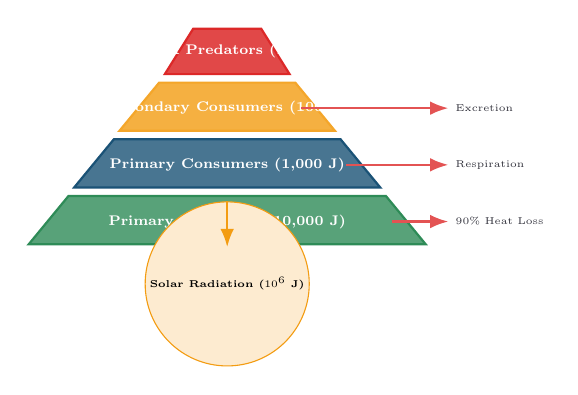
\begin{tikzpicture}[font=\sffamily, scale=0.72, transform shape]
                % Level 4: Apex Predators
                \draw[fill=accent!85, draw=accent, thick] (-1.1, 3.1) -- (1.1, 3.1) -- (0.6, 3.9) -- (-0.6, 3.9) -- cycle;
                \node[text=white, font=\bfseries\scriptsize] at (0, 3.5) {Apex Predators (10 J)};
                
                % Level 3: Secondary Consumers
                \draw[fill=midorange!80, draw=midorange!90, thick] (-1.9, 2.1) -- (1.9, 2.1) -- (1.2, 2.95) -- (-1.2, 2.95) -- cycle;
                \node[text=white, font=\bfseries\scriptsize] at (0, 2.5) {Secondary Consumers (100 J)};
                
                % Level 2: Primary Consumers
                \draw[fill=journalblue!80, draw=journalblue, thick] (-2.7, 1.1) -- (2.7, 1.1) -- (2.0, 1.95) -- (-2.0, 1.95) -- cycle;
                \node[text=white, font=\bfseries\scriptsize] at (0, 1.5) {Primary Consumers (1,000 J)};
                
                % Level 1: Primary Producers
                \draw[fill=donegreen!80, draw=donegreen, thick] (-3.5, 0.1) -- (3.5, 0.1) -- (2.8, 0.95) -- (-2.8, 0.95) -- cycle;
                \node[text=white, font=\bfseries\scriptsize] at (0, 0.5) {Primary Producers (10,000 J)};
                
                % Dissipation Arrows
                \draw[-Latex, thick, draw=accent!80] (2.9, 0.5) -- ++(1.0, 0) node[right, font=\tiny, text=structure]{$90\%$ Heat Loss};
                \draw[-Latex, thick, draw=accent!80] (2.1, 1.5) -- ++(1.8, 0) node[right, font=\tiny, text=structure]{Respiration};
                \draw[-Latex, thick, draw=accent!80] (1.3, 2.5) -- ++(2.6, 0) node[right, font=\tiny, text=structure]{Excretion};
                
                % Solar Input
                \node[circle, draw=midorange, fill=midorange!20, inner sep=2pt, font=\tiny\bfseries] (sun) at (0, -0.6) {Solar Radiation ($10^6$ J)};
                \draw[-Latex, thick, draw=midorange] (sun) -- (0, 0.05);
            \end{tikzpicture}
            \par\vspace{2pt}
            {\tiny\textcolor{structure!70}{Fig 1: Scalable vector trophic energy tier model.}}
        \end{column}
    \end{columns}
\end{frame}

% --- Slide 5: Michaelis-Menten & Hill Enzyme Kinetics ---
\section{Kinetics}
\begin{frame}{Enzymatic Kinetics: Michaelis-Menten \& Hill Cooperativity}
    \begin{columns}[c]
        \begin{column}{0.48\textwidth}
            \pillalt{HILL COOPERATIVITY}\par\vspace{0.2em}
            \scriptsize
            Cooperative substrate-ligand binding velocity:
            \begin{equation*}
                v = \frac{V_{\max} [S]^h}{K_{0.5}^h + [S]^h}
            \end{equation*}
            \vspace{0.1em}
            \begin{itemize}\setlength{\itemsep}{1.5pt}
                \item \textbf{Hill Coefficient ($h$):}
                \begin{itemize}\setlength{\itemsep}{1pt}
                    \item $h > 1$: Positive cooperativity (Sigmoidal curve).
                    \item $h = 1$: Standard Michaelis-Menten (Hyperbolic).
                    \item $h < 1$: Negative cooperativity.
                \end{itemize}
                \item \textbf{Half-Saturation ($K_{0.5}$):} Concentration at $v = \frac{1}{2} V_{\max}$.
            \end{itemize}
        \end{column}
        \begin{column}{0.48\textwidth}
            \pill{POPULATION DYNAMICS}\par\vspace{0.2em}
            \scriptsize
            Lotka-Volterra Predator-Prey Coupled ODEs:
            \begin{align*}
                \frac{dN}{dt} &= rN - aNP \quad \text{(Prey)} \\
                \frac{dP}{dt} &= baNP - mP \quad \text{(Predators)}
            \end{align*}
            \vspace{0.1em}
            \begin{takeaway}
                \textbf{Ecological Equilibrium:} Non-trivial fixed point occurs at $(N^*, P^*) = \left(\frac{m}{ba}, \frac{r}{a}\right)$.
            \end{takeaway}
        \end{column}
    \end{columns}
\end{frame}

% --- Slide 6: Kinetic Parameters Summary Table ---
\section{Parameters}
\begin{frame}{Enzymatic Parameters \& Catalytic Efficiency}
    \begin{columns}[c]
        \begin{column}{0.56\textwidth}
            \centering
            \setlength{\tabcolsep}{4.0pt}
            \scriptsize
            \begin{tabular}{@{} l c c c @{}}
                \toprule
                \rowcolor{tableheader}
                \textbf{Enzyme System} & \textbf{$K_m$ ($\mu\mathrm{M}$)} & \textbf{$k_{\mathrm{cat}}$ ($\mathrm{s}^{-1}$)} & \textbf{$k_{\mathrm{cat}}/K_m$ ($\mathrm{M}^{-1}\mathrm{s}^{-1}$)} \\
                \midrule
                Carbonic Anhydrase & $12{,}000$ & $1{,}000{,}000$ & $8.3 \times 10^7$ \\
                Acetylcholinesterase & $95$ & $14{,}000$ & $1.5 \times 10^8$ \\
                Triose Phosphate Isomerase & $470$ & $4{,}300$ & $9.1 \times 10^6$ \\
                Catalase & $25{,}000$ & $40{,}000{,}000$ & $1.6 \times 10^9$ \\
                \bottomrule
            \end{tabular}
            \par\vspace{3pt}
            {\tiny\textcolor{structure!70}{Catalytic efficiency approaching the diffusion-controlled limit ($10^8\text{--}10^9\,\mathrm{M}^{-1}\mathrm{s}^{-1}$).}}
        \end{column}
        \begin{column}{0.42\textwidth}
            \pillalt{KINETIC METRICS}\par\vspace{0.3em}
            \scriptsize
            \begin{itemize}\setlength{\itemsep}{2pt}
                \item \textbf{Turnover Number ($k_{\mathrm{cat}}$):} Maximum substrate molecules converted per active site per second.
                \item \textbf{Specificity Constant ($k_{\mathrm{cat}}/K_m$):} Measure of catalytic perfection.
                \item \textbf{Diffusion Limit:} Upper bound imposed by Brownian molecular collisions.
            \end{itemize}
        \end{column}
    \end{columns}
\end{frame}

% --- Slide 7: Python Code Listing ---
\begin{frame}[fragile]{Numerical Simulation of Lotka-Volterra Systems}
\begin{lstlisting}[language=Python, basicstyle=\ttfamily\scriptsize, keywordstyle=\color{accent}\bfseries, commentstyle=\color{structure!60}\itshape, stringstyle=\color{journalblue}, frame=single, rulecolor=\color{structure!20}, backgroundcolor=\color{structure!3}, numbers=left, numberstyle=\tiny\color{structure!50}]
import numpy as np
from scipy.integrate import odeint

def lotka_volterra_dynamics(state: list, t: float, r: float, a: float, b: float, m: float):
    """Computes time derivatives for coupled predator-prey populations."""
    N, P = state
    dN_dt = r * N - a * N * P
    dP_dt = b * a * N * P - m * P
    return [dN_dt, dP_dt]

# Integrate trajectory
t_span = np.linspace(0, 50, 1000)
initial_state = [40.0, 9.0]
params = (0.5, 0.02, 0.1, 0.2)
trajectory = odeint(lotka_volterra_dynamics, initial_state, t_span, args=params)
\end{lstlisting}
\end{frame}

% --- Slide 8: Summary ---
\section{Summary}
\begin{frame}{Key Biophysical Takeaways}
    \begin{columns}[t]
        \begin{column}{0.48\textwidth}
            \pill{SUMMARY}\par\vspace{0.3em}
            \begin{itemize}\setlength{\itemsep}{2.5pt}
                \item \textbf{Trophic Tiers:} Thermodynamic loss constrains ecosystem depth.
                \item \textbf{Enzyme Kinetics:} Hill cooperativity models non-linear allosteric transitions.
                \item \textbf{Dynamic Stability:} Predator-prey phase orbits oscillate around center equilibria.
            \end{itemize}
        \end{column}
        \begin{column}{0.48\textwidth}
            \pillalt{NEXT STEPS}\par\vspace{0.3em}
            \begin{itemize}\setlength{\itemsep}{2.5pt}
                \item \textbf{Lab Session 4:} Measure alkaline phosphatase $K_m$ and $V_{\max}$.
                \item \textbf{Problem Set 3:} Derive Lineweaver-Burk linear transformations.
                \item \textbf{Office Hours:} Monday 15:00--17:00 (Bio Lab 108).
            \end{itemize}
            \vspace{0.3em}
            \begin{takeaway}
                \textbf{Contact:} \texttt{bio-instructor@university.edu}
            \end{takeaway}
        \end{column}
    \end{columns}
\end{frame}

% --- Slide 9: References ---
\begin{frame}[allowframebreaks]{References}
    \printbibliography
\end{frame}

\end{document}
